% Template for PLoS
% Version 3.5 March 2018
%
% % % % % % % % % % % % % % % % % % % % % %
%
% -- IMPORTANT NOTE
%
% This template contains comments intended
% to minimize problems and delays during our production
% process. Please follow the template instructions
% whenever possible.
%
% % % % % % % % % % % % % % % % % % % % % % %
%
% Once your paper is accepted for publication,
% PLEASE REMOVE ALL TRACKED CHANGES in this file
% and leave only the final text of your manuscript.
% PLOS recommends the use of latexdiff to track changes during review, as this will help to maintain a clean tex file.
% Visit https://www.ctan.org/pkg/latexdiff?lang=en for info or contact us at latex@plos.org.
%
%
% There are no restrictions on package use within the LaTeX files except that
% no packages listed in the template may be deleted.
%
% Please do not include colors or graphics in the text.
%
% The manuscript LaTeX source should be contained within a single file (do not use \input, \externaldocument, or similar commands).
%
% % % % % % % % % % % % % % % % % % % % % % %
%
% -- FIGURES AND TABLES
%
% Please include tables/figure captions directly after the paragraph where they are first cited in the text.
%
% DO NOT INCLUDE GRAPHICS IN YOUR MANUSCRIPT
% - Figures should be uploaded separately from your manuscript file.
% - Figures generated using LaTeX should be extracted and removed from the PDF before submission.
% - Figures containing multiple panels/subfigures must be combined into one image file before submission.
% For figure citations, please use "Fig" instead of "Figure".
% See http://journals.plos.org/plosone/s/figures for PLOS figure guidelines.
%
% Tables should be cell-based and may not contain:
% - spacing/line breaks within cells to alter layout or alignment
% - do not nest tabular environments (no tabular environments within tabular environments)
% - no graphics or colored text (cell background color/shading OK)
% See http://journals.plos.org/plosone/s/tables for table guidelines.
%
% For tables that exceed the width of the text column, use the adjustwidth environment as illustrated in the example table in text below.
%
% % % % % % % % % % % % % % % % % % % % % % % %
%
% -- EQUATIONS, MATH SYMBOLS, SUBSCRIPTS, AND SUPERSCRIPTS
%
% IMPORTANT
% Below are a few tips to help format your equations and other special characters according to our specifications. For more tips to help reduce the possibility of formatting errors during conversion, please see our LaTeX guidelines at http://journals.plos.org/plosone/s/latex
%
% For inline equations, please be sure to include all portions of an equation in the math environment.
%
% Do not include text that is not math in the math environment.
%
% Please add line breaks to long display equations when possible in order to fit size of the column.
%
% For inline equations, please do not include punctuation (commas, etc) within the math environment unless this is part of the equation.
%
% When adding superscript or subscripts outside of brackets/braces, please group using {}.
%
% Do not use \cal for caligraphic font.  Instead, use \mathcal{}
%
% % % % % % % % % % % % % % % % % % % % % % % %
%
% Please contact latex@plos.org with any questions.
%
% % % % % % % % % % % % % % % % % % % % % % % %

\documentclass[10pt,letterpaper]{article}
\usepackage[top=0.85in,left=2.75in,footskip=0.75in]{geometry}

% amsmath and amssymb packages, useful for mathematical formulas and symbols
\usepackage{amsmath,amssymb}

% Use adjustwidth environment to exceed column width (see example table in text)
\usepackage{changepage}

% Use Unicode characters when possible
\usepackage[utf8x]{inputenc}

% textcomp package and marvosym package for additional characters
\usepackage{textcomp,marvosym}

% cite package, to clean up citations in the main text. Do not remove.
% \usepackage{cite}

% Use nameref to cite supporting information files (see Supporting Information section for more info)
\usepackage{nameref,hyperref}

% line numbers
\usepackage[right]{lineno}

% ligatures disabled
\usepackage{microtype}
\DisableLigatures[f]{encoding = *, family = * }

% color can be used to apply background shading to table cells only
\usepackage[table]{xcolor}

% array package and thick rules for tables
\usepackage{array}

% create "+" rule type for thick vertical lines
\newcolumntype{+}{!{\vrule width 2pt}}

% create \thickcline for thick horizontal lines of variable length
\newlength\savedwidth
\newcommand\thickcline[1]{%
  \noalign{\global\savedwidth\arrayrulewidth\global\arrayrulewidth 2pt}%
  \cline{#1}%
  \noalign{\vskip\arrayrulewidth}%
  \noalign{\global\arrayrulewidth\savedwidth}%
}

% \thickhline command for thick horizontal lines that span the table
\newcommand\thickhline{\noalign{\global\savedwidth\arrayrulewidth\global\arrayrulewidth 2pt}%
\hline
\noalign{\global\arrayrulewidth\savedwidth}}


% Remove comment for double spacing
%\usepackage{setspace}
%\doublespacing

% Text layout
\raggedright
\setlength{\parindent}{0.5cm}
\textwidth 5.25in
\textheight 8.75in

% Bold the 'Figure #' in the caption and separate it from the title/caption with a period
% Captions will be left justified
\usepackage[aboveskip=1pt,labelfont=bf,labelsep=period,justification=raggedright,singlelinecheck=off]{caption}
\renewcommand{\figurename}{Fig}

% Use the PLoS provided BiBTeX style
% \bibliographystyle{plos2015}

% Remove brackets from numbering in List of References
\makeatletter
\renewcommand{\@biblabel}[1]{\quad#1.}
\makeatother



% Header and Footer with logo
\usepackage{lastpage,fancyhdr,graphicx}
\usepackage{epstopdf}
%\pagestyle{myheadings}
\pagestyle{fancy}
\fancyhf{}
%\setlength{\headheight}{27.023pt}
%\lhead{
\includegraphics[width=2.0in]{PLOS-submission.eps}}
\rfoot{\thepage/\pageref{LastPage}}
\renewcommand{\headrulewidth}{0pt}
\renewcommand{\footrule}{\hrule height 2pt \vspace{2mm}}
\fancyheadoffset[L]{2.25in}
\fancyfootoffset[L]{2.25in}
\lfoot{\today}

%% Include all macros below

\newcommand{\lorem}{{\bf LOREM}}
\newcommand{\ipsum}{{\bf IPSUM}}





\usepackage{forarray}
\usepackage{xstring}
\newcommand{\getIndex}[2]{
  \ForEach{,}{\IfEq{#1}{\thislevelitem}{\number\thislevelcount\ExitForEach}{}}{#2}
}

\setcounter{secnumdepth}{0}

\newcommand{\getAff}[1]{
  \getIndex{#1}{}
}

\providecommand{\tightlist}{%
  \setlength{\itemsep}{0pt}\setlength{\parskip}{0pt}}

\begin{document}
\vspace*{0.2in}

% Title must be 250 characters or less.
\begin{flushleft}
{\Large
\textbf\newline{CEEDS Weather Dashboard} % Please use "sentence case" for title and headings (capitalize only the first word in a title (or heading), the first word in a subtitle (or subheading), and any proper nouns).
}
\newline
% Insert author names, affiliations and corresponding author email (do not include titles, positions, or degrees).
\\
Julia Lee\textsuperscript{},
Marta García\textsuperscript{},
Mirella Hernandez\textsuperscript{}\\
\bigskip
\bigskip
\end{flushleft}
% Please keep the abstract below 300 words
\section*{Abstract}
The MacLeish Field Station is open to all the Smith College community,
and the field station contains and captures a lot of weather data and
historical information, such as precipitation, temperature, and wind
speed. Thus, the station currently has a weather dashboard where all the
information and data from the year 2012 of the field is collected and
displayed. Despite there being an existing MacLeish weather dashboard,
the MacLeish Field Station manager, Paul Wetzel, wants to update the
weather dashboard to better showcase the weather data for the public to
feel more inclined to download the MacLeish weather data and overall use
the dashboard. Therefore, we primarily focused on creating the updated
MacLeish weather dashboard to be more user friendly by incorporating
interactive graphics and allowing users to download and filter the data.
We created a Shiny App to update the dashboard, so we used ``shiny'' and
``shiny dashboard'' packages in R as well as HTML and CSS to build and
interactive dashboard.

% Please keep the Author Summary between 150 and 200 words
% Use first person. PLOS ONE authors please skip this step.
% Author Summary not valid for PLOS ONE submissions.

\linenumbers

% Use "Eq" instead of "Equation" for equation citations.
\section{Introduction}\label{introduction}

The Center for the Environment, Ecological Design, and Sustainability
(CEEDS) is located in Wright Hall building of Smith College. The
Macleish Field Station is a part of CEEDS, and students are able to
conduct research, work on environmental projects, and overall explore
the field there. The MacLeish Field Station is located near Whately,
Massachusetts, and its weather collection sites are at the end of Poplar
Hill Road (footnote/cite current MacLeish weather dashboard). There are
two weather site locations in the field, one called WhatelyMet tower and
the other tower is called OrchardMet. The WhatelyMet tower is 25.3
meters tall and it is slightly further away from the center of the field
station, since it was initially created to collect air pollution data.
In order to collect more efficient weather data on ground level,
OrchardMet weather station was created. Despite this, the trees do not
allow OrchardMet weather station to collect data efficiently as hoped.

As part of the SDS 410 Capstone class, we worked with Paul Wetzel, the
MacLeish field station manager, in updating the current MacLeish weather
dashboard. The current MacLeish weather dashboard collects a variety of
weather data: date, wind speed, temperature, wind direction, real
humidity, pressure, solar radiation, and rainfall. The server has been
collecting data since January 2012 through WhatelyMet tower, and it has
been collecting additional weather data since 2015 through OrchardMet
tower. The data is updated every 10 minutes; thus, there is over 377,016
entries. The data loggers run on solar power and stores the data so even
if the server is down the data is saved.

The current MacLeish weather dashboard\footnote{current Macleish weather
  dashboard: http://macleish.smith.edu/index.html} contains a lot of
useful information, and the data is organized into readable tabs (see
fig. 1). Our client, Paul, is the currently the one who uses it the most
and understands it. Despite this, Paul wants to update the MacLeish
weather dashboard for others in addition to himself to better access and
use the MacLeish weather data and its dashboard. Therefore, the focus we
chose for this project is to recreate the current Macleish weather
dashboard to better showcase the data and make it more user friendly by
keeping its tab structure, adding visually interactive graphs, and
allowing users to download and filter data as proposed by Paul. We chose
to create a Shiny App when updating the MacLeish weather dashboard, so
we used ``shiny'' and ``shiny dashboard'' packages. We choose to use
Shiny, since it would allow us to make the download data opportunity
catered to the audience's needs, it would help us make the graphs
interactive, and it be more user friendly. We believe our focus would
supply to the current target audiences, Paul Wetzel, other Smith
students, Smith faculty/researchers, and Northampton Department of
Public Works.

\begin{figure}
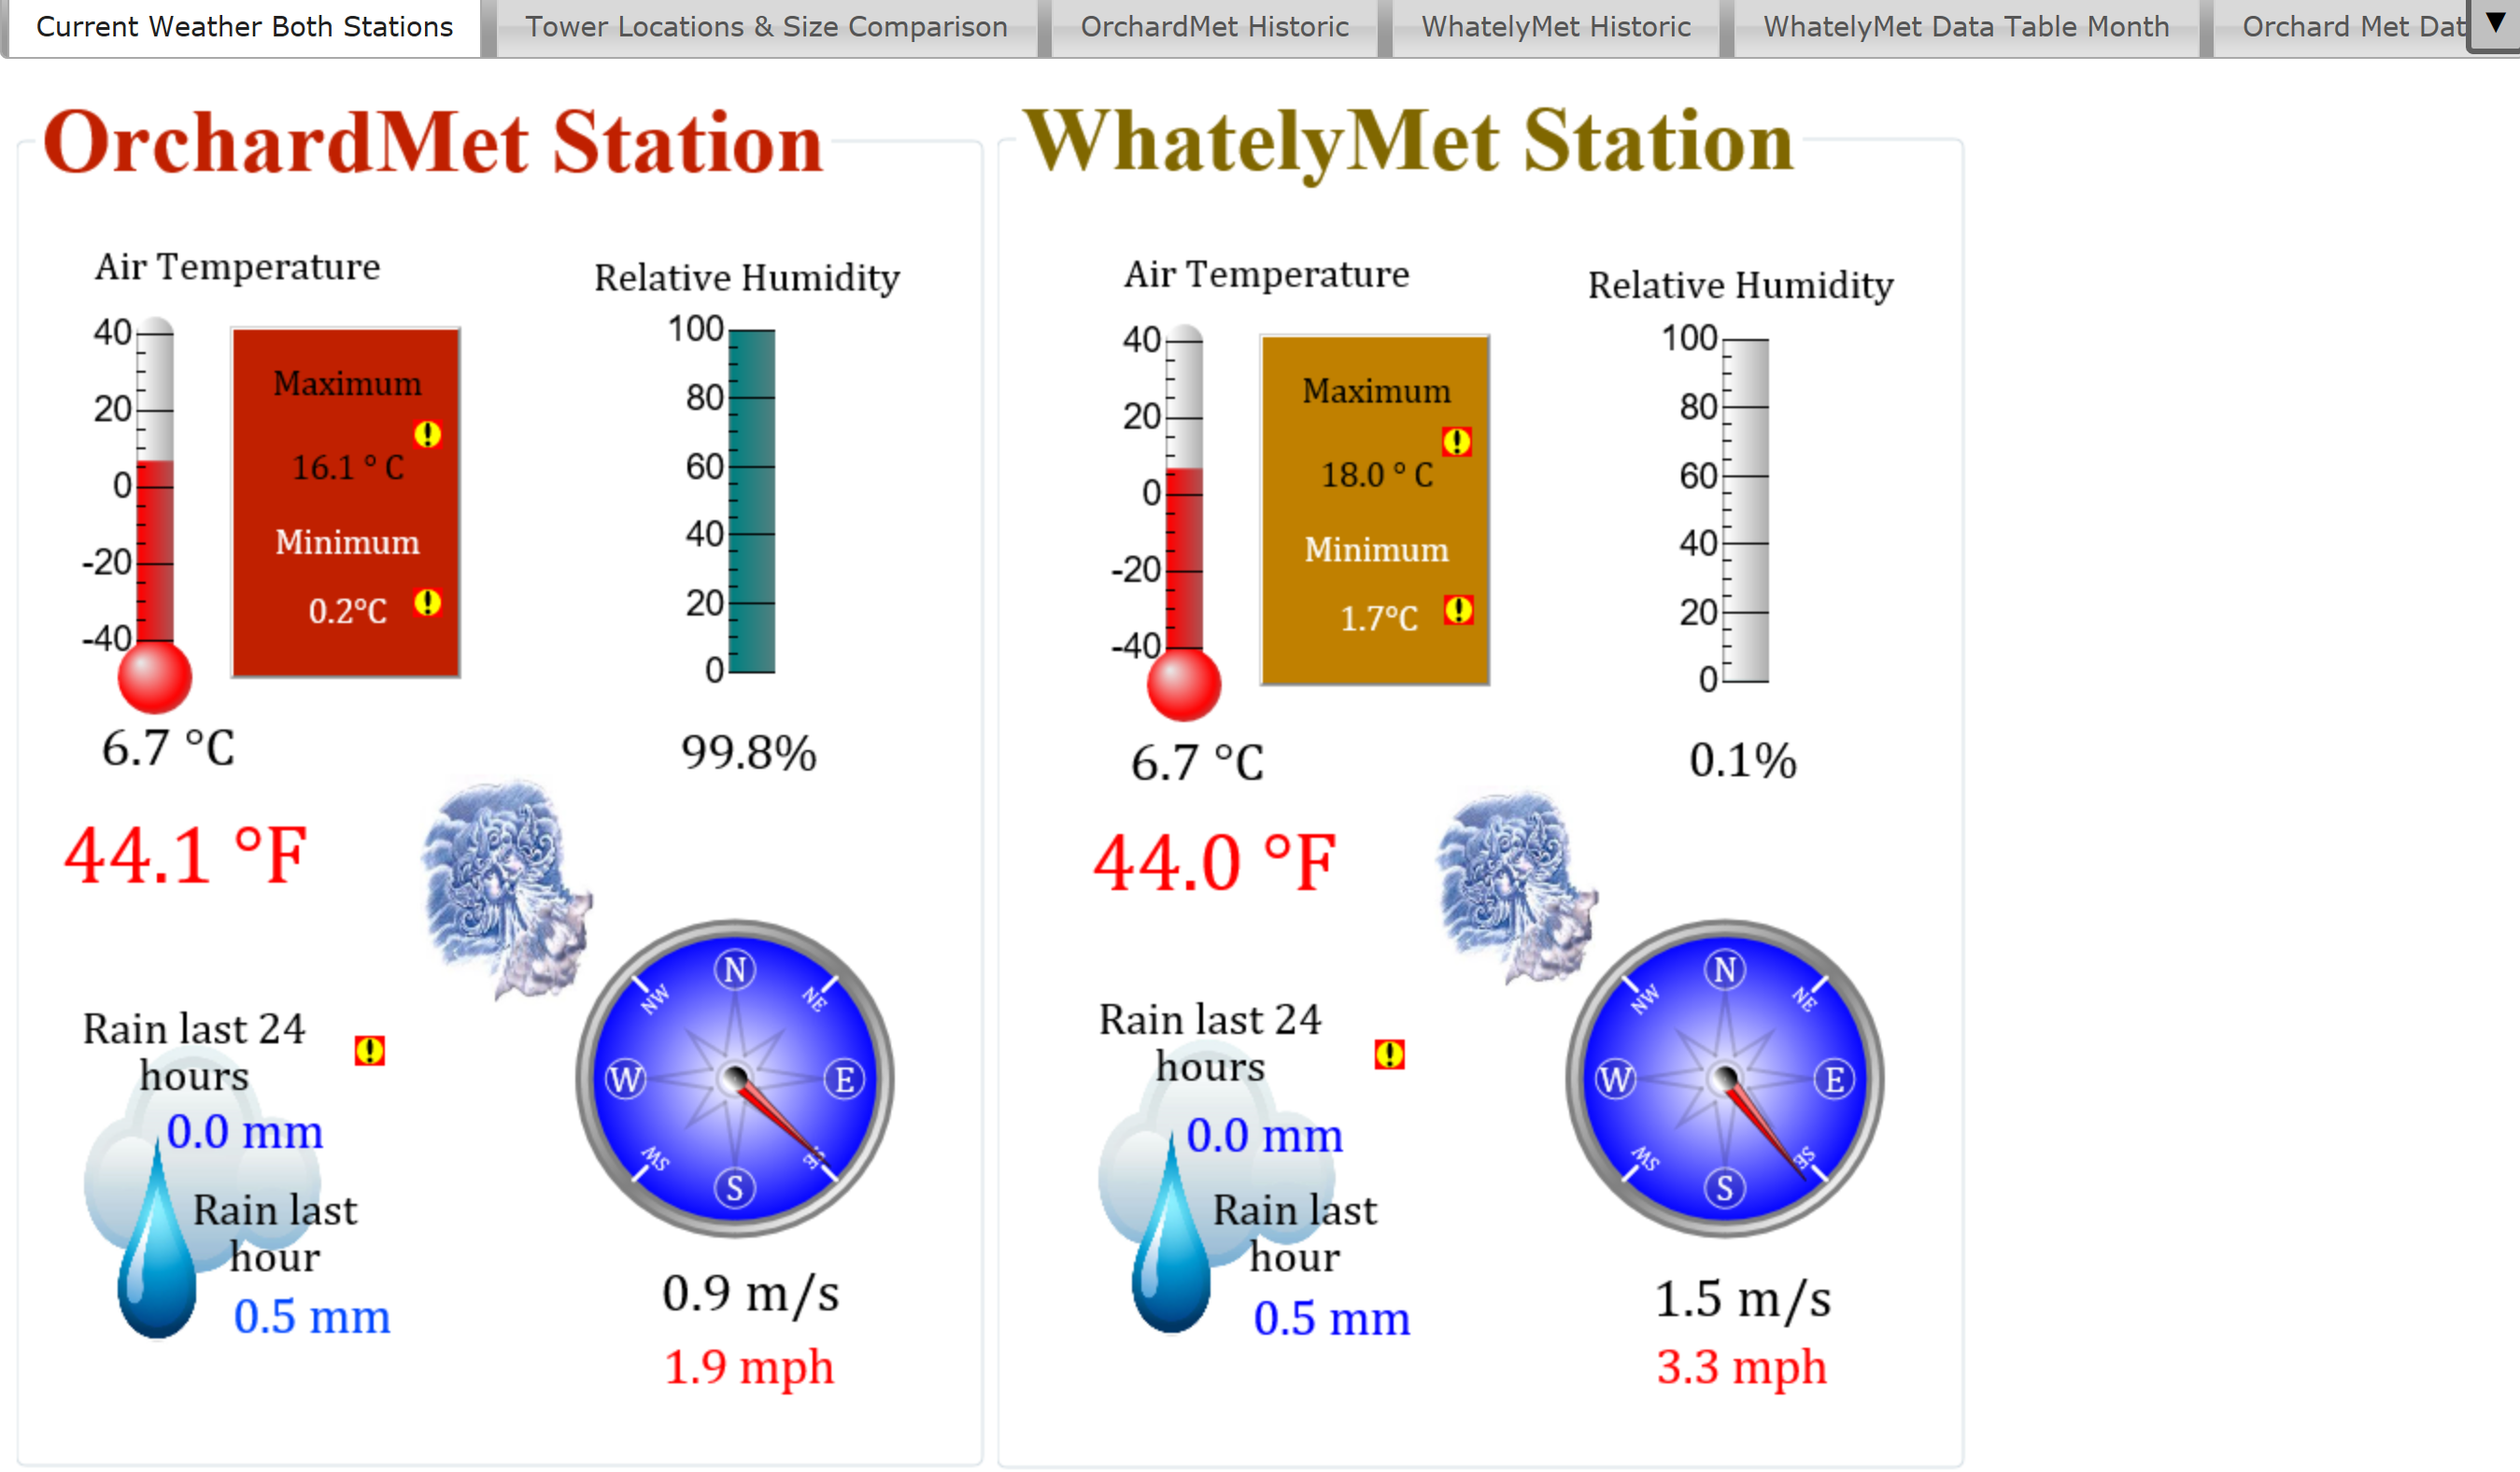
\includegraphics[width=350px]{current} \caption{fig 1: Example of a what the current Macleish weather dashboard looks like}\label{fig:unnamed-chunk-1}
\end{figure}

\section{Methods}\label{methods}

\subsection{Shiny app:}\label{shiny-app}

To solve our problem, we had many options on how to create a better way
of displaying the weather data. We first discussed the possibility of
making a new website in html but we ultimately decided to build a Shiny
App using the Shiny and Shiny Dashboard packages in R. Shiny is a
package that allows us ``to build interactive web applications (apps)
straight from R.'' Shiny allows the user to be able better communicate
data with interactive charts, visualizations, text and tables. We then
decided to use Shiny Dashboard which is a package that allows us to
create an interactive dashboard, an informative platform that visually
collects, analyzes, and displays data, using Shiny. Because our problem
was to find a way to display interactive data visualizations, the Shiny
package seemed to be the better option because that is what it was built
to do. Shiny also allows us to make normally static plots like ggplots
interactive and take in user input so we don't need to use html widgets.

Shiny is based on a reactive programming model which means that it takes
in input given by the user of the app and acts accordingly. Shiny apps
have two components: the user interface (UI) and the server. You can
think of the UI as what the user of your app will see when they open
your app. The UI component converts your code in R and generates it into
a web document in html. UI contains the instruction about what you want
the user to see and the layout of your app. Our UI is where we define
the dashboard page. Inside the dashboard page, we define our elements
like the sidebar menu, tabs, the dashboard body (tab items, boxes,
text). The server is the R code that tells your shiny server what to do
when the user does certain things in the app. The server is a function
where we define the output and tell the host of our app what to do with
the user input. Server function is also where we render the charts,
visualizations, and tables. We then knit together the Server function
and UI using the ShinyApp (UI, server) function in the Shiny package.

\subsection{Current Weather Tab:}\label{current-weather-tab}

Thus, we built a Shiny dashboard. Our dashboard has a sidebar menu that
has four tab items: current weather, about, historical data, and
download data. We chose to focus on these 4 tab items since it answers
to our client's primary needs. The first tab we built and have displayed
as the main page of the weather dashboard is the current weather tab
(see fig. 2). The current weather tab gives the user the current 10
minute weather for WhatelyMet and OrchardMet. Because we wanted to have
our data be shown as a text object and not a table, our code for this
tab was largely done using html. Additionally to address our clients
need of having the MacLeish weather dashboard be more user friendly, we
chose to design the weather tab in a minimalist style. By doing so, the
users will be able to better see the data in one glimpse.

\section{\texorpdfstring{\texttt{\{r,echo=FALSE,\ fig.cap=\ "fig\ 2:\ Current\ Weather\ Tab\ displaying\ WhatelyMet\ and\ OrchardMet\ current\ weather\ and\ showing\ how\ our\ sidebar\ menu\ and\ dashboard\ looks\ like",\ out.width\ =\ "350px"\}\ \#\ knitr::include\_graphics("")\ \#}}{\{r,echo=FALSE, fig.cap= "fig 2: Current Weather Tab displaying WhatelyMet and OrchardMet current weather and showing how our sidebar menu and dashboard looks like", out.width = "350px"\} \# knitr::include\_graphics("") \#}}\label{rechofalse-fig.cap-fig-2-current-weather-tab-displaying-whatelymet-and-orchardmet-current-weather-and-showing-how-our-sidebar-menu-and-dashboard-looks-like-out.width-350px-knitrinclude_graphics}

\subsection{About Tab:}\label{about-tab}

The second tab we built on our dashboard is the about tab, which is
where we explained our project and have information about the weather
stations (see fig 3). We also added links for the public to contact Paul
for further questions and interests as well as our repository link. This
tab was created as the updated version of the ``Tower Locations \& Size
Comparisons'' tab in the current MacLeish Dashboard to better
communicate with the users. We used a bit of HTML to change the sizing
of the text and the alignment of the rows. To make the teal boxes, we
used the shinydashboard Plus package {[}1{]}, allowed us to make a
clear, concise first page of our Shiny app.

\section{\texorpdfstring{\texttt{\{r,\ echo=FALSE,\ fig.cap="fig\ 3:\ Welcoming\ the\ users\ and\ letting\ them\ know\ who\ to\ reach\ out\ to\ for\ further\ information\ and\ how\ the\ app\ works",\ out.width\ =\ "350px"\}\ \#\ knitr::include\_graphics("")\ \#}}{\{r, echo=FALSE, fig.cap="fig 3: Welcoming the users and letting them know who to reach out to for further information and how the app works", out.width = "350px"\} \# knitr::include\_graphics("") \#}}\label{r-echofalse-fig.capfig-3-welcoming-the-users-and-letting-them-know-who-to-reach-out-to-for-further-information-and-how-the-app-works-out.width-350px-knitrinclude_graphics}

\subsection{Historic Data Tab:}\label{historic-data-tab}

The third tab we built was the historic data tab (see fig 4). This tab
is the updated version of the ``OrchardMet Historic'' and ``WhatelyMet
Historic'' of the current MacLeish weather dashboard. When building this
tab, we focused on displaying the weather data through visual
interactive graphs as our client requested. We made a way for the user
to switch between daily data for OrchardMet and WhatelyMet in the
historic data tab, this means the graphs shown are reactive and are
based on the data set that was selected by the user. We did this by
making a reactive function inside the server that allows people to
switch between data sets. We made graphs mapping 3 of our client's focus
variables (Wind speed, precipitation, temperature) over time (see fig
5). To build these graphs, we used the Highcharter package {[}2{]} that
allows the user to filter the data based on a certain time period and
high charter also has a feature that enables users to download the data
used to make the graphic.

\section{\texorpdfstring{\texttt{\{r,\ echo=FALSE,\ fig.cap="fig\ 4:\ The\ way\ the\ Historic\ Data\ tab\ looks\ and\ how\ it\ allows\ the\ users\ to\ choose\ what\ weather\ station\ they\ would\ like\ to\ look\ at",\ out.width\ =\ "350px"\}\ \#\ knitr::include\_graphics("")\ \#}}{\{r, echo=FALSE, fig.cap="fig 4: The way the Historic Data tab looks and how it allows the users to choose what weather station they would like to look at", out.width = "350px"\} \# knitr::include\_graphics("") \#}}\label{r-echofalse-fig.capfig-4-the-way-the-historic-data-tab-looks-and-how-it-allows-the-users-to-choose-what-weather-station-they-would-like-to-look-at-out.width-350px-knitrinclude_graphics}

\begin{figure}
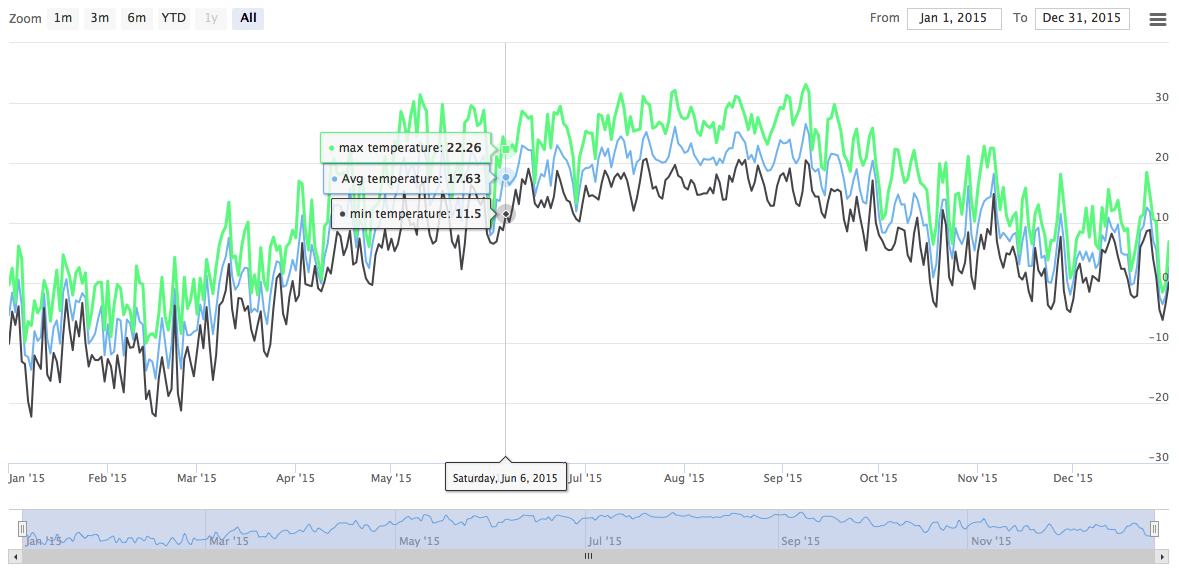
\includegraphics[width=350px]{highchart} \caption{fig 5:Example of a Highcharter graph that shows temperature}\label{fig:unnamed-chunk-2}
\end{figure}

We also made a visualization where the user can make a custom
correlation graph by picking the variables that they want. We made this
correlation scatterplot by using ggplot and ggplotly to make the graphic
more interactive. We also made a windrose graph to show wind speed and
direction using ggplot (see fig 6). A wind rose is a polar chart which
shows the user how wind speed and wind direction are distributed at a
over a specific period of time. We also created a way to allow the user
to choose a variable and get summary statistics on that variable. In
this tab, we made the graphs be in a fluid page, this allows for the
size of the boxes and visuals to change based on the size of the window.
We then put all of our content for the tab in separate boxes that are
collapsible. We did this to minimize users' scrolling.

\begin{figure}
\includegraphics[width=350px]{windrose} \caption{fig 6: A wind rose graph}\label{fig:unnamed-chunk-3}
\end{figure}

\subsection{Dowloand Data Tab}\label{dowloand-data-tab}

Since our client wanted users to be able to download and filter the
MacLeish weather data that is displayed in the dashboard, we added a new
tab, raw data tab, which the current MacLeish weather dashboard does not
have. This tab allows the user to filter the data based on columns and
the user can also choose between daily data for OrchardMet and
WhatelyMet (see fig 7). This tab also allows the user to search the data
table using the DT package.

\section{\texorpdfstring{\texttt{\{r,\ echo=FALSE,\ fig.cap="fig\ 7:\ The\ way\ dowloading\ data\ tab\ looks,\ and\ how\ it\ allows\ users\ to\ filter\ the\ data\ they\ would\ like\ to\ download",\ out.width\ =\ "350px"\}\ \#\ knitr::include\_graphics("")\ \#}}{\{r, echo=FALSE, fig.cap="fig 7: The way dowloading data tab looks, and how it allows users to filter the data they would like to download", out.width = "350px"\} \# knitr::include\_graphics("") \#}}\label{r-echofalse-fig.capfig-7-the-way-dowloading-data-tab-looks-and-how-it-allows-users-to-filter-the-data-they-would-like-to-download-out.width-350px-knitrinclude_graphics}

\subsection{Ceeds package:}\label{ceeds-package}

The data from the two weather stations is currently being saved on the
Macleish Server hosted at Smith college. We used the Macleish package to
fetch the two data tables from the server. However this involved a lot
of code that would have to be repeated anytime we wanted to run the app.
So we decided to write an R package to more efficiently do these tasks.
This package was also built to help other students to work on the
MacLeish weather data. We wrote a function that uses the Macleish
package and fetches 2 data sets (Whately, Orchard) that is updated every
ten minutes. We also created a function,get\_daily(), inside the package
that takes a data set and gives the user the data grouped by date. Our
data from the server comes in 10 minute increments but we might want to
group by date. So we used the Lubridate package was very helpful. It
allowed us to Parsed timestamps into dates (turning variables into dates
that r can recognize as such). This allowed us to group our data by
date. {[}3{]}

\section{Issues}\label{issues}

Throughout this whole process, our group has faced a variety of issues
and consequently, temporary limitations. At the beginning of our
process, we first had to learn to use the Shiny package. There was a
learning curve in learning to build a web app and we initially struggled
with building the first parts of the app and figuring out how to
integrate the R knowledge we had with this new package. We took the
DataCamp course to learn the basics of Shiny and from there, dove
straight into our new data, once we had access to the data. Since we
were reliant on the MacLeish package, which relied on the MacLeish
server to receive the data, whenever the MacLeish server was down, we
struggled with working with the data we needed to move forth with the
project.

Also at the start of this project, we met with our client to gather more
information of what he wanted and what we felt we could deliver knowing
our skill set in R and Shiny. Since Wetzel was not familiar with the
capabilities of R, it was up to us to fill him in with what we thought
was possible. These plans included reducing the amount of tabs, changing
all the graphs to being clearly interactive, and making the web app
overall more user-friendly and comprehensive. We did not create a
printed mockup until much later in the process so it was difficult to
communicate our vision to him and for him to understand the potential of
R and Shiny. However, in our biweekly meetings with him, we filled him
in with whatever progress we were making and once we started creating
visualizations using highcharter, he was able to better understand the
kind of graphs we could create and integrate into the new web app.

In the similar vein as to how Wetzel did not know much about R, our
group did not know much about weather data and the importance of all the
variables. During our meeting Wetzel taught us the importance of certain
variables but also told us that we should focus on the precipitation,
temperature and wind variables if we needed to narrow our scope. In
teaching us about the other variables, such as soil temperature and
server temperature and this helped us figure out which variables were
most important to the user. For example, the server room temperature
would be most useful to the weather station manager (Wetzel) because
that temperature would allow him to see when the room was overheating or
too cold, and not very functional for a user looking to download weather
data for a school project. Through Wetzel, we also learned that
temperature data is only accurate up to the thousandth place which made
us modify our app to reflect that accuracy.

Arguably our largest and most time-consuming issue, making tabs work in
Shiny took a while. Since our project is so visual, and tabs played a
major part in our functioning dashboard, this set us back and we were
unable to move forward with the HTML \& CSS coding until we could solve
this problem. We had already programmed in some graphs but with tabs not
working, they would all appear on the same page and when the user tried
to click to different tabs, they would not switch. However, with some
help from our professor Ben Baumer, we were able to get tabs to work.
Through this, we learned the importance of correct placement of commas
and parentheses in Shiny since as we discovered later, that had been our
problem the whole time. Once tabs worked, we were able to put all the
appropriate graphs in each tab and start working on the user interface
that we coded mostly with HTML \& CSS.

A smaller issue that we had was making graphs reactive. Since we were so
familiar with using ggplot package through tidyverse, we wanted to have
all our data visualizations be programmed using ggplot. However, we had
a lot of issues with making these visualizations reactive with Shiny,
which posed a problem of how a user would then interact with these
graphs. After trying for a short while, we ultimately moved onto a
different package called highcharter, which made the graphs interactive
and also allowed an element of downloading data that we expanded on
later with a tab we included. We also faced issues when building the tab
that allowed users to download data and making images show up in the
about tab. Both of these issues were solved by continuously trying new
methods over and over again, but specifically solved the issue with
images by installing the package base64enc since the problem was about
different directories and file paths that were not accessible by all
machines.

\section{Moving Forward}\label{moving-forward}

There are many things that can looked at in future to expand this
project. A future endeavor of our project is that we have not yet
surveyed our target audience about whether our app is more usable than
the current dashboard. Audience feedback would help us moving forward in
reach our end goal of creating a user friendly weather dashboard. We
have already tested our dashboard with a group of peers, however we
would like to test on a wider audience.

After talking to our client, we found out that sometimes the weather
equipment breaks which leads to inaccuracy in the data it records. Due
to this, Wetzel often goes in and manually changes the data. We don't
necessarily want to filter out possible outliers of the data (assuming
that they mean equipment malfunctions), but we would have liked to
either include a small disclaimer that would tell people downloading or
analyzing the data about this or include both the raw and corrected
data. That way, users can reach that conclusion on their own just by
comparing the two datasets.

We would have also liked to implement some sort of special setting that
would have extra tabs for our client, the weather manager. These extra
tabs would include data that is important to him, such as soil
temperature and the bunker room temperature, both tabs we felt were not
important to our general audience of students and others looking to
check the weather or download a large amount of data. A variable like
soil temperature is used to study climate change so while it may not
seem important immediately, with context, it could prove to be a
valuable variable to study and analyze.

\section*{References}\label{references}
\addcontentsline{toc}{section}{References}

{[}4{]}

\hypertarget{refs}{}
\hypertarget{ref-dashboardplus}{}
1. Granjon D. ShinydashboardPlus: Add more 'adminlte2' components to
'shinydashboard' {[}Internet{]}. 2019. Available:
\url{https://CRAN.R-project.org/package=shinydashboardPlus}

\hypertarget{ref-highcharter}{}
2. Kunst J. Highcharter: A wrapper for the 'highcharts' library
{[}Internet{]}. 2019. Available:
\url{https://CRAN.R-project.org/package=highcharter}

\hypertarget{ref-ceeds}{}
3. Baumer BS, García M, Hernandez M, Lee J. Ceeds. 2019.

\hypertarget{ref-ceeds_repo}{}
4. Baumer BS, García M, Hernandez M, Lee J. Ceeds github repository.
\url{https://github.com/beanumber/ceeds}; 2019.

\nolinenumbers


\end{document}

